% https://tex.stackexchange.com/a/445105
\documentclass{beamer}
\usepackage[english]{babel}
\usepackage{ragged2e}
%\usepackage{utopia} %font utopia imported
%\usepackage{graphicx} %package to manage images
\usepackage[utf8]{inputenc}
\usepackage[T1]{fontenc}
\usepackage{blkarray, bigstrut}
%\usepackage[utf8]{inputenc}%codification of the document
\usepackage{tikz}
\usetheme{Warsaw}
\usecolortheme{beaver}
\usetikzlibrary{decorations.markings}

\title[Module 8]{MODULE 8 \\ Data Matrix : Generation }
\author[aa]{by\texorpdfstring{\\}{}aa}
\setbeamertemplate{page number in head/foot}[totalframenumber]


\begin{document}

\begin{frame}
\frametitle{Re-numbered 2-D grid}
\begin{center}
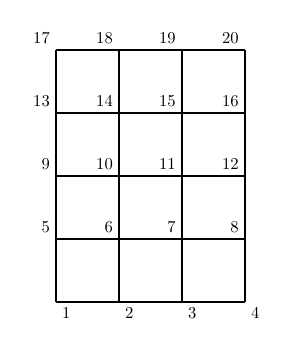
\begin{tikzpicture}[thick,scale=0.4, every node/.style={scale=0.6}]

\draw (0,0) grid[step=2cm] (6,8);
\foreach \X [count=\x] in {0,...,3} 
{\foreach \Y [count=\y] in {0,...,4}
 {
 \ifnum\Y=0
  \node[anchor=north west] at (2*\X,2*\Y) {\x};
 \else
   \node[anchor=south east] at (2*\X,2*\Y) {\number\numexpr\x+\Y*4};
 \fi
 }
}
\end{tikzpicture}
\hspace{3cm}
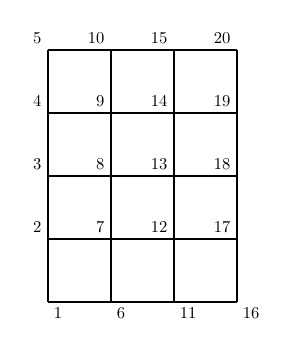
\begin{tikzpicture}[thick,scale=0.4, every node/.style={scale=0.6}]

\draw (0,0) grid[step=2cm] (6,8);
\foreach \X [count=\x] in {0,...,3} 
{\foreach \Y [count=\y] in {0,...,4}
 {
 \ifnum\Y=0
  \node[anchor=north west] at (2*\X,2*\Y) {\number\numexpr(\x-1)*5+1};
 \else
  \node[anchor=south east] at (2*\X,2*\Y) {\number\numexpr(\x-1)*5+\Y+1};
 \fi
 }
}
\end{tikzpicture}
\end{center}
\end{frame}
\end{document}
